\documentclass[twoside,10pt]{article}
\usepackage{shlists}
\usepackage[applemac]{inputenc}
\usepackage[spanish]{babel}
\usepackage[T1]{fontenc}


\usepackage{multicol}
\usepackage{picinpar}

\usepackage{url}
\newcommand{\surl}[1]{{\small\url{#1}}}

\newcounter{vol}
\newcounter{num}
\newcounter{anyo}
\setcounter{vol}{9}
\setcounter{num}{1}
\setcounter{anyo}{2016}
\newcommand{\mes}{Enero}
\usepackage{revisionNLcol}


\title{\ \\ Docencia 2.0\\ \large Juan Juli\'an Merelo, Fernando Tricas}
\author{\LARGE El miedo a fallar}

\date{}

\AutTit{Docencia 2.0}

\begin{document}
\addtocounter{page}{2}

\maketitle
\vspace*{-2ex}

\begin{multicols}{2}
 
En general, en la ense\~{n}anza universitaria de la programaci\'{o}n y tareas
aleda\~{n}as, como administraci\'{o}n de sistemas, se ense\~{n}a a acertar: a que
tu c\'{o}digo compile correctamente, pase todos los \textsl{tests} y finalmente
haga lo que tiene que hacer. Los contenidos, ejercicios y pr\'{a}cticas se
encaminan a que no haya ning\'{u}n fallo en ese proceso.

Pero en ingenier\'{\i}a las cosas no siempre van como a uno le gustar\'{\i}a que
fueran. En cualquier paso en el proceso de creaci\'{o}n de un sistema
inform\'{a}tico, un espacio mal colocado o un punto y coma omitido y el
ordenador expulsa una parrafada, muchas veces en ingl\'{e}s,
expresando su impotencia y su falta de comprensi\'{o}n por lo que el ser
humano est\'{a} intentando hacer. Y el problema es que, cada vez m\'{a}s, el
ser humano matriculado en un grado de ingenier\'{\i}a, ante esa parrafada,
s\'{o}lo sabe expresar su impotencia y su 
falta de comprensi\'{o}n al profesor de teor\'{\i}a o pr\'{a}cticas m\'{a}s cercano. 

�\textsl{Use the force, Luke}� dec\'ia el maestro al aprendiz en aquella saga
que se ha puesto de moda otra vez durante las \'ultimas semanas. Y a
pesar de que tambi\'en aqu\'el otro dec\'ia aquello de �\textsl{The force is
strong with this one!}�, lo cierto es que el protagonista no dejaba de
utilizar por ello las herramientas que ten\'ia disponibles: la espada
l\'aser, las naves y los robots, por ejemplo. 

!`Incluso se entrenaba para aprender a manejarlas adecuadadamente! 

As\'i que ser\'a nuestra tarea intentar convencer a nuestros
estudiantes del valor de los mensajes de error: nuestro compilador favorito (o
para el caso, de alguien) nos lanza mensajes y notificaciones que var\'ian
mucho en calidad y claridad cuando hemos cometido alg\'un errorcillo. En muchos
casos nos ayudar\'{a}n a hacernos una idea de lo que est\'a pasando y en otros nos
dar\'an por lo menos alguna pista de por d\'onde tenemos que empezar a mirar. 

Por eso, pedimos a los j\'{o}venes {\em padawanes} que practiquen las siguientes
virtudes teologales de un desarrollador cuando aparecen los errores: 

\begin{itemize}
\item Fe: el compilador sabe (o, m\'{a}s bien, no sabe otra cosa). Si se queja es
que algo hemos hecho mal (no encuentra lo que esperaba encontrar).  
Y nos avisa.
\item Esperanza: todo tiene remedio. Revisemos la l\'inea donde nos
  se\~nalan, desde el principio de la lista de errores, y sus
  alrededores. A veces ayuda dejarlo un rato y volver m\'as tarde. No
  ayuda volver a hacer exactamente lo mismo a ver si pillamos
  despistado al compilador y se le olvida darnos el mismo error. 
\item Caridad: siempre encontraremos quien nos ayude. O a qui\'en
  ayudar. El c\'odigo fuente tiene la rara {\em virtud} de
  confundirnos cuando lo miramos fijamente. Nuevas miradas y ojos nuevos son
inmunes a esta confusi\'{o}n, a veces.  
\end{itemize}

Y que, una vez practicadas y alcanzado el zen con ellas 
%--------------------------
\noindent\rule{86mm}{1pt}
\vspace{1ex} {\small{\begin{window}[0,r,
\includegraphics[width = 27
mm]{JJM.jpg},] \noindent\emph{JJ Merelo} es catedr\'{a}tico de Universidad
en el \'area de Arquitectura y Tecnolog\'{\i}a de Computadores, y
actualmente director de la Oficina de Software Libre de la UGR.
Mantiene un blog desde el a\~no 2002, y lo ha utilizado en clase desde
el a\~no 2004; tambi\'en wikis y, ultimamente, agregadores y otras
herramientas TIC. \'{U}ltimamente le ha dado por el \textsl{flipped
learning}, de lo que se informar\'{a} debidamente en esta columna.
\end{window}}}

\medskip

{\small{\begin{window}[0,r,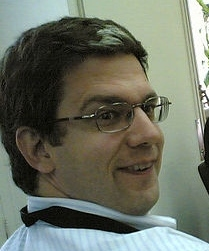
\includegraphics[width = 27 mm]{FTricas1.jpg},]
		\noindent  \emph{Fernando Tricas Garc\'{\i}a} es profesor
		titular de Lenguajes y Sistemas Inform\'aticos del Departamento
		de Inform\'atica e Ingenier\'{\i}a de Sistemas de la Universidad de
		Zaragoza.  Empez\'o a estudiar la blogosfera casi cuando a\'un no
		exist\'{\i}a (all\'a por el a\~no 2002) y a tratar de integrarla en los
		cursos y tareas docentes un poco despu\'es.  Ha impartido
		numerosas charlas relacionadas con el tema de la Web 2.0.
		Es actualmente Director de su departamento.  
		\end{window}}}
%-------------------------------------------------

\noindent (�\textsl{The force awakens}�), se pueden complementar con las virtudes
cardinales. 
\begin{itemize}
\item Prudencia. Una copia de seguridad, o un ``commit'' 
a tiempo y una
  nueva rama, para probar cambios sin destrozar ninguna
  funcionalidad. A ver si arreglando algo se nos va a estropear lo
  dem\'as. 
\item Justicia. El compilador no tiene la culpa. El computador
  tampoco, ni el que nos encarg\'o la pr\'actica. Especialmente el que
  nos encarga la pr\'{a}ctica.
\item Fortaleza. El que resiste gana. Y las herramientas son muy
  robustas, pero\ldots\ ?`Dejaremos que nos venzan unas pocas l\'ineas de
  c\'odigo? 
\item Templanza. A\~nadir otra opci\'on a nuestro programa no lo hace
  mejor. Incluir las \'ultimas caracter\'isticas de la \'ultima
  versi\'on del lenguaje, tampoco. El objetivo es resolver la
  funcionalidad que sea necesaria y, de paso, aprender cosas
  interesantes. A veces tenemos la tentaci\'on de modificar c\'odigo,
  a\~nadir l\'ineas y duplicar funciones para resolver errores. 
\end{itemize}

Lo importante es hacerlo. Como dijo Yoda, �\textsl{Do. Or do not. There is no
try.}� Si lo intentas y no funciona, vuelve a intentarlo hasta que
funcione. 

Para terminar, �\textsl{And may the Force be with you!}�. La fuerza es, sin duda,
StackOverflow, donde preguntar y contestar ayudar\'{a} a tu karma. No hay
duda que StackOverflow no resuelva, si ya ha fallado el grupo de
WhatsApp de clase, el profesor de pr\'{a}cticas que sabe siempre m\'{a}s que
el de teor\'{\i}a y el que sac\'{o} m\'{a}s de un ocho el a\~{n}o anterior en la misma asignatura. Raro es el
error que no le ha ocurrido a alguien, en alg\'{u}n lugar, alguna vez. Y
esa persona, muy probablemente, lo haya resuelto y lo haya puesto en
alg\'{u}n lado. Simplemente busca y encontrar\'{a}s, joven padawan.  
\bigskip

\noindent\emph{Todas las columnas de la serie Docencia 2.0
pueden descargarse en formato LaTeX desde
\surl{https://github.com/ReVision-Docencia-20/Columnas}}

\noindent\rule{90mm}{1pt}

{\small \noindent\copyright 2016 JJ. Merelo, F. Tricas. Este art\'{\i}culo es de acceso libre distribuido bajo los t\'erminos
de la Licencia Creative Commons de Atribuci\'on, que permite copiar,
distribuir y comunicar p\'ublicamente la obra en cualquier medio, s\'olido
o electr\'onico, siempre que se acrediten a los autores y fuentes
originales}

\end{multicols}
\end{document}
	








\end{multicols}
\end{document}
